\documentclass{standalone}
\usepackage{tikz}

\begin{document}
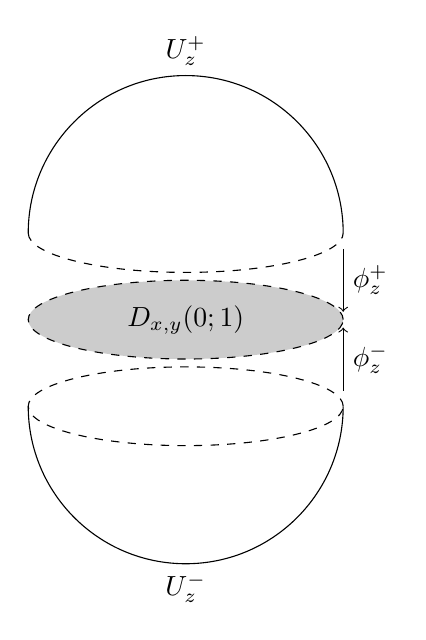
\begin{tikzpicture}
	\draw[dashed] (-2,0) arc[start angle=180, end angle=360, x radius=2, y
		radius=0.5];
\draw (2,0) arc[start angle=0, end angle=180, radius=2] node[midway, above]{$
	U_z^+ $};

\draw[->] (2,-0.2) -- (2,-1) node[midway, right]{$ \phi_z^+ $};

\filldraw[dashed, fill=gray!50, fill opacity=0.8] (0,-1.1) ellipse (2 and 0.5);
\draw (0,-1.1) node{$ D _{x,y}(0;1) $};

\draw[dashed] (0,-2.2) ellipse (2 and 0.5);
\draw (2,-2.2) arc[start angle=0, end angle=-180, radius=2] node[midway, below]{$
	U_z^- $};
\draw[->] (2,-2) -- (2,-1.2) node[midway, right]{$ \phi_z^- $};
\end{tikzpicture}
\end{document}

